\documentclass[modern]{aastex631}


\usepackage{amsmath}
\usepackage{amssymb}
\usepackage{hyperref}
\usepackage{bm}
\usepackage{listings}
\usepackage{graphicx}
\usepackage{float}
\usepackage{soul}
\usepackage{mathtools}
\usepackage{esint}

% missing figure command

\usepackage{blindtext}
\usepackage{graphicx}
\usepackage{tcolorbox}
\usepackage{fontawesome}
\usepackage{booktabs}

\definecolor{linkcolor}{rgb}{0.1216,0.4667,0.7059}


\let\StandardIncludeGraphics\includegraphics%
\renewcommand{\includegraphics}[2][]{%
\IfFileExists{#2}{%
  \StandardIncludeGraphics[#1]{#2}%
}{%
 \IfFileExists{#2.pdf}{%
  \StandardIncludeGraphics[#1]{#2}%
  }{ % No, no .pdf, try *.jpg 
   \IfFileExists{#2.jpg}{%
    \StandardIncludeGraphics[#1]{#2}%
    }{
      \IfFileExists{#2.png}{%
      \StandardIncludeGraphics[#1]{#2}%
      }{%
      \begin{tcolorbox}[width=6cm,height=4cm,arc=0mm,auto outer arc]
      \end{tcolorbox}
     }
   }
 }
}% 
%
}

% commands
\newcommand{\todo}[1]{\colorbox{red}{\textcolor{white}{\texttt{TO DO}}}\,}
\newcommand{\set}[1]{\{\,#1\,\}}
\newcommand{\footlink}[1]{\footnote{\url{#1}}}
\DeclareMathOperator*{\argmax}{arg\,max}
\DeclareMathOperator*{\argmin}{arg\,min}
\let\subsectionautorefname\sectionautorefname
\let\subsubsectionautorefname\sectionautorefname
\newcommand{\codeicon}{{\color{linkcolor}\faFileCodeO}}
\newcommand{\codelink}[1]{\href{https://github.com/lgrcia/paper-jaxoplanet/blob/main/#1.py}{\codeicon}\,\,}
\newcommand{\gitlink}{\href{https://github.com/lgrcia/paper-jaxoplanet}{\color{linkcolor}\faGithub}\,\,}

% no indent
\setlength\parindent{0pt}

% code style
\lstdefinestyle{mystyle}{
    backgroundcolor=\color{white},
    commentstyle=\color{gray!70},
    keywordstyle=\color{Bittersweet},
    stringstyle=\color{RoyalBlue},
    basicstyle=\fontsize{8.5}{13}\fontfamily{DejaVuSansMono-TLF}\selectfont,
    breakatwhitespace=false,         
    breaklines=true,
    rulecolor=\color{black!15},
    numbers=none,
    numberstyle=\fontsize{7}{11}\fontfamily{DejaVuSansMono-TLF}\selectfont\color{gray!50},
    framerule=0pt,
    breakindent=5pt,
    resetmargins=true,
    numbersep=10pt,
    frame=single,
    aboveskip=1em,
    belowskip=1em,
    xleftmargin=6pt,
    framexleftmargin=4pt
}
\lstset{style=mystyle}

\newcommand{\bvec}[1]{{\ensuremath{\mathbf{#1}}}}

\begin{document}

\title{\textsf{jaxoplanet}: Hardware-Accelerated Computation of Stellar Light Curves}

% author info
\author{Lionel J. Garcia}
\author{Soichiro Hattori}
\author{Daniel Foreman-Mackey}
\affiliation{Center for Computational Astrophysics, Flatiron Institute, New York, NY, USA}

\keywords{}

\begin{abstract}
    Modeling light curves of extrasolar systems serves a wide variety of science cases. Transit and occultation light curves, for example, are used to characterize their orbital configuration, and infer the atmospheric properties of their transiting bodies. Phase curves, on the other hand, can be used to study the thermal emission of exoplanets, and the atmospheric circulation of stars. In order to infer these properties, a fast, accurate and robust model of stellar light curves is needed, one that accounts for the non-uniform surface intensity of spherical bodies and their mutual occultations. In this context, the analytical framework known as \textsf{starry} provided the community with a powerful tool, instrumental in .... However, as datasets and models complexity grow, the tractable inference of these parameters becomes increasingly challenging, and often motivates biased approximations. In this paper, we present a new implementation of the \textsf{starry} framework in \texttt{jax}, a high-performance machine-learning library designed for large-scale computations. We describe the changes made to the original version of \textsf{starry} and evaluate the performance of its new implementation that we release in the open-source Python package \textsf{jaxoplanet}. Through this implementation, we provide the community with a differentiable model of stellar light curves, and enable the use of powerful machine-learning tools available in the \textsf{JAX} ecosystem. \gitlink{}

\end{abstract}

\section{Introduction}

Planets of the solar system used to be known and studied through their position in the sky. It is only starting in the 16th century that Earth-based telescopes progressively enabled the direct imaging of their surface. But despite these new instruments, some minor planets were too small and too distant to be imaged, and remained unresolved until the end of the 20th century, when more capable space-based observatories were launched. This is the case of Pluto, for example, whose surface was first studied thanks to the light it reflects while rotating and orbiting the Sun. Using point source observations obtained from 1945 to 1986, \cite{Drish1995} tentatively reconstructed the map of the planet, and only later compared it to the first \textit{Hubble Space Telescope} low-resolution images obtained by \cite{Stern1997}. This mapping effort was gloriously completed with the extremely detailed pictures obtained by the \textit{New Horizons} spacrecraft during its fly-by of the planet \citep{Stern2015}.\\\\
Although imaging the surface of an exoplanet might be several decades away, their study follows that of Pluto, by first employing indirect methods and unresolved light curves (see \citealt{Mayor1995} and \citealt{Charbonneau2000})  while waiting for the development of more powerful direct imaging instruments \cite{}. Similarly, stellar photospheres can currently be mapped using interferometry and Doppler imaging, but these techniques are costly and can only be applied to a handful of objects, so that time-resolved spectrophotometry remains our main way to study them. In this context, the development of accurate and robust models of stellar light curves is crucial.\\\\
In the age of wide-field surveys (such as) and high-precision spectroscopic instruments, these models are being compared to large datasets in probabilistic ways, requiring fast and robust evaluations of their posterior likelihood over larger and larger parameter spaces. These inferences can be highly facilitated by gradient-based optimization and sampling algorithms, so that being able to differentiate these models with respect to their parameters offers clear advantages.\\\\
In this context, \cite{starry} and \cite{Agol2020} presented a framework to analytically compute the light curves of spherical bodies with non-uniform surface intensities, such as stars and exoplanets, and the flux observed from their mutual occultations. This framework, known as \textit{starry}, has been successfully applied to a wide variety of science cases, like the study of transiting exoplanets \citep{Kostov2019}, precise modeling of radial velocities \citep{Dawson2021}, the study of exoplanets atmospheres \citep{Bell2023} or the study of stellar photospheres \citep{Almenara2022}. However, as datasets and models complexity grow, the tractable inference of the larger parameter spaces we have to deal with becomes increasingly challenging, and often motivates biased approximations. This is the case, for example, in transmission spectroscopy measurements conducted with the \textit{James Webb Space Telescope} NIRSpec instrument, that should ideally consist in the simultaneous modeling of more than 3000 transit light curves, one per pixel element (e.g. \citealt{Alderson2023}).\\\\
In this paper we present \textsf{jaxoplanet}, a new implementation of the \textit{starry} framework in \texttt{JAX}, a high-performance machine-learning library designed for large-scale computations, including autodifferentiation capabilities, deployed on various hardware. In \autoref{starry}, we summarize the formalism introduced by \cite{starry} to analytically compute stellar light curves. In \autoref{optimization}, we describe the \textsf{jaxoplanet} implementation and the changes made to the \textsf{starry} implementation. Finally, in \autoref{performance}, we evaluate the performance of our new implementation that we release in the open-source Python package \textsf{jaxoplanet}. Through this implementation, we provide the community with a differentiable model of stellar light curves, and enable the use of powerful machine-learning tools available in the \texttt{JAX} ecosystem.\\\\





% the computation of \textit{starry} light curves can be computationally expensive, especially when considering the large number of parameters that need to be inferred from the data. In this paper, we present a new implementation of the \textit{starry} model that leverages the \texttt{jax} library to perform hardware-accelerated computations on GPUs. We show that this implementation can be used to compute light curves up to 100 times faster than the original implementation, and we demonstrate its application to the inference of the orbital parameters of exoplanets from transit light curves.



% Stellar light curves and radial velocity models provided an important tool to study exoplanetary systems. At the origin of these models lies the first principles of orbital mechanics, the Kepler equations, and the algorithms used to solve them. On top of that, models like Agol, of occultation light curves extended our capability to study these systems in greater details, using transits. In practice, computing this model and making inference based on these observables has been enabled by the implementation of these models with optimized frameworks and inference tools (pymc3), providing robust implementation of sampling algorithms and other inferrence tools. A good example of this synergy is the development of exoplanet and starry in c++ backed by Pymc3 which enabled major discoveries based on large datasets. With the recent lunch of JWST, we crumble under data. For example, transmission spectra on hundreds of channels, multi-planet systems and a large number of free parameters with their priors. At the same time, machine learning continue to grow, and novel framework appear and lead to application in physics. One of this framework is jax, developped by google, and gaining a huge popularity on the astronomy community. JAX is a hp machine-learning library that pre-compile code to LAX for paralilisation. It allows complex model to be written direclty in python, where usually a lower-level langage like C is preferable, and parallelised on CPU, GPU or any lax-compatible device. Not only it's good because of the higher level syntax of python that made it popular in science. But also because of the capability to run expansive models on GPU, a trend observed in other field of ML and DL where scaling is required.

% In this paper, we describe an implementation of the starry formalism in jax, allowing for the inference of a large number of parameters on complex models, exploiting the latest dev in ML machinery.

\section{Light curve models}\label{starry}

Inspired by the idea of \cite{pal2012}, \cite{starry} and \cite{Agol2020} present a general framework to compute the light curves of spherical bodies with non-uniform surface intensities. In this section, we describe the mathematical formalism behind the \textit{starry} model.

\subsection{Spherical harmonics}

The surface of a spherical body can be naturally described by spherical harmonics: a set of special functions defined on the sphere that can serve as orthonormal basis to represent any spherical surface map. If $\bvec{\tilde y}$ denotes the spherical harmonics basis of degree $l_{max}$ (defined in \citealt[section 2.2]{starry}) and $\bvec{y}$ a vector that contains the coefficients describing the surface in this basis, the intensity $I$ of the map projected onto the sky-projected $(x, y)$ plane of the observer is
\begin{equation}I(x, y) = \bvec{\tilde y^\mathsf{T}}(x, y) \, \bvec{y}.\end{equation}
In order to orient this surface, for example with a given inclination, obliquity and phase around its rotation axis, we define a rotation matrix $\bvec{R}$ that acts on the spherical harmonics coefficients $\bvec{y}$, such that the intensity of the map projected onto the sky of the observer is
\begin{equation}I(x, y) = \bvec{\tilde y}^\mathsf{T}(x, y) \, \bvec{R} \, \bvec{y}.\end{equation}\\
\subsection{Rotation light curve}
Using this expression, the integrated intensity of the rotated map is
\begin{equation}F = \iint I(x,y)\,\text{d}S = \iint \bvec{\tilde y^\mathsf{T}}\bvec{R}\bvec{y}\,\text{d}S\end{equation}
In order to simplify this integral, \citealt{starry} introduce a change of basis from the spherical harmonics basis $\bvec{\tilde y}$ to a simple polynomial basis $\bvec{\tilde p}$ (defined in \citealt[section 2.3]{starry}) characterized by the change of basis matrix $\bvec{A_1}$. In this new basis, $\bvec{y}$ can be expressed as
\begin{equation}\bvec{p} = \bvec{A_1}\bvec{y},\end{equation}
such that 
\begin{equation}I(x, y) = \bvec{\tilde p^\mathsf{T}}(x, y)\,\bvec{A_1}\bvec{R}\bvec{y}.\end{equation}
Hence,
\begin{equation}F = \iint \bvec{\tilde p^\mathsf{T}}\bvec{A_1}\bvec{R}\bvec{y}\,\text{d}S = \bvec{r^\mathsf{T}}\bvec{A_1}\bvec{R}\bvec{y},\end{equation}
with
\begin{equation}\bvec{r^\mathsf{T}} \equiv \iint \mathbf{\tilde{p}}^\top\,\text{d}S,\end{equation}
since $\bvec{A_1}$, $\bvec{R}$ and $\bvec{y}$ are independent of the coordinates on the sphere.\\\\
As $\bvec{\tilde{p}}$ is simply made of polynomials of the coordinates $x$, $y$ and $z$, the elements of the \textit{rotation vector} $\bvec{r}^\mathsf{T}$ can be computed analytically and only once for a given $l_{max}$ (see \citealt[Eq. 20]{starry}).\\\\
\subsection{Occultation light curve}\label{occultation}
In order to model transits and occultations, the same formalism can be used to compute the integrated intensity of a surface map occulted by another spherical body. In this case, the intensity of the map must be integrated only over the unocculted surface $S$ of the disk, such that 
\begin{equation} F = \iint_S I(x,y)\,\text{d}S = \left(\iint_S \bvec{\tilde p^\mathsf{T}}\,\text{d}S\right)\bvec{A_1}\bvec{R}\bvec{y}.\end{equation}
To simplify this expression, \cite{pal2012} note that any two-dimensional integral of the unocculted disk can be reduced to a one-dimensional integral over the contour $C$ of the occulting body using Green's theorem\footnote{Also known as Stokes' theorem in three-dimensional vector calculus.}. This can be done if the integrand of the integral over S can be described by a function $f$ such that
\begin{equation}f(x, y) = \frac{\delta G_{y}}{\delta x}-\frac{\delta G_{x}}{\delta y},\end{equation}
where $G$ is a vector field defined and differentiable over $S$.\\\\
By applying a last change of basis matrix $\bvec{A_2}$ to the polynomial basis $\bvec{\tilde p}$, \cite{starry} transforms $\bvec{\tilde p}$ to the \textit{Green's basis} $\bm{\tilde g}$ that satisfies this property, meaning that the surface integral of each of its components $\tilde{g_n}$ can be transformed to the line integral
\begin{equation}
    \label{eq:sn_gn}
    s_n \equiv \iint_S \tilde{g_n}(x, y)\,\text{d}S = \oint_C \bvec{G}_n(x, y)\,\text{d}\bvec{r},
\end{equation}
with $\bvec{G}_n$ given in \citealt[Equation 34]{starry}. These functions require the occulting body to be aligned with the $y$-axis of the reference frame, which can be achieved by applying a final rotation matrix $\bvec{R'}$ to the surface map.\\\\
Using these expressions, the integrated intensity of the occulted map follows the idiomatic linear expression 
\begin{equation}
    \label{eq:starry}
    F = \bvec{s^\mathsf{T}}\bvec{A}\,\bvec{R'}\,\bvec{R}\,\bvec{y},
\end{equation}
with $\bvec{A} = \bvec{A_2A_1}$ and the integrals $s_n$ arranged in the \textit{solution vector} $\bvec{s^\mathsf{T}}$.\\\\

\subsection{Limb-darkened surfaces}
We notice that a simpler situation is encountered when the surface of the spherical body can be described by a radial intensity profile $I(r)$, such as a limb-darkened star. In this case, the vector of spherical harmonics coefficients $\bvec{y}$ is very sparse (because all $m\neq0$ components are zero) and the surface map doesn't need to be rotated. Contemporary to \cite{starry}, \cite{Agol2020} explore this case and provide simple expressions for the integrated intensity of a star whose surface can be described by a polynomial limb darkening law occulted by an opaque body. In this case:
\begin{enumerate}
    \item The surface is simply described by $\bvec{u}$, a vector of polynomial limb darkening coefficients.
    \item The Green's basis takes a simpler form (see \citealt[Equation 14]{Agol2020}).
    \item Matrices involved in the computation of the integrated flux have $l_{max}$ columns, versus $(l_{max}+1)^2$ in the general case, reducing drastically the computational cost of the model.
\end{enumerate}
For these reasons, and because of its wide application, our implementation treats radially-symmetric maps separately, leading to highly optimize computations of limb-darkened light curves.\\\\


\newpage
\section{Implementation details}\label{optimization}
The formalism introduced by \cite{starry}, summarized in \autoref{starry}, provides an elegant analytical model of stellar light curves. Implemented in C++ and released in the \texttt{starry} Python package, it was built for the probabilistic programming library \textsf{PyMC3} and led to several advances in the field of exoplanetary science. However, since its initial development, the \textsf{PyMC} project adopted several breaking changes that made \textsf{starry} incompatible with its latest versions. Updating \textsf{starry} to the latest version of \textsf{PyMC} would require a complete rewriting of the code, that would again be highly dependent on the latter. Hence, our first motivation comes from the broken dependencies of \textsf{starry} and aims to provide the community with an implementation compatible with a wider ecosystem of tools. In this respect \textsf{JAX} represents an interesting alternative. This high-performance machine-learning library can be used to perform hardware-accelerated computations on various type of devices (CPU, GPU, TPU) and gave rise to probabilistic tools developped by an ever-growing community of scientists and engineers. However, \textsf{JAX} capabilities really shine when models are written with a functional-programming mindset, and computations performed in a vectorized way.\\\\
In this section, we describe the changes made to the original \textsf{starry} implementation to allow its rewriting in \textsf{JAX}. We also highlight details about the latest version of \textsf{starry}'s original implementation that were omitted in \citealt{starry} but described in parts of its code and documentation. 

\subsection{Limb darkened maps}
Limb darkened maps are obtained by multiplying a base map, devoid of limb darkening, with a pure limb darkened map. If $\bvec{U}$ is the change of basis matrix that transforms the polynomial limb darkening coefficients $\bvec{u}$ to the spherical harmonics coefficients $\bvec{y}_u$, the pure limb darkened map is
\begin{equation}
    \label{eq:limb_darkening_map}
    \bvec{y}_u = \bvec{U}\bvec{u}.
\end{equation}
The multiplication of the base map represented by $\bvec{y}$ with the limb darkening map represented by $\bvec{y}_u$ can be seen as the multiplication of two polynomials, only with special coefficients (called Clebsch–Gordan coefficients) inherent to the properties of spherical harmonics. To simplify this operation, we transform both maps into the polynomial basis, so that their product is the actual product of two polynomials which doesn't require the computation of special coefficients.

\subsection{Limb darkening normalization}
In \textsf{starry} version 0.2.2 \citep{starry}, the normalization of a limb-darkened light curve was done by assuming that adding limb darkening to a non-uniform surface does not modify its total luminosity. Hence, the total flux received from a star during its complete rotation should be the same with or without limb darkening. In older versions of starry ($\le$0.2.2), this was done by actually computing the light curve of the star with and without limb darkening, and using the ratio of the two to normalize the limb darkened light curve. As discussed in the \textsf{starry} documentation\footlink{https://starry.readthedocs.io/en/latest/notebooks/LDNormalization/} this approach is wrong and leads to an unphysical normalization.\\\\
Instead, one can assume that the total flux of the star should be similar for all observers, independently of the surface map of the star. In addition to the fact that all components of the spherical harmonics basis integrate to 0 (except the constant component $Y_{0,0}$) we deduce that the mean flux of the star must be coming from a static surface seen by any observer, no matter his viewpoint, which corresponds to a purely limb-darkened surface (with no other source of non-uniformity).\\\\
The flux of this purely limb-darkened surface is
\begin{equation}
    f_u = \bvec{r}^\mathsf{T}\bvec{A_1}\bvec{y}_u
\end{equation}
with $\bvec{y}_u$ defined in \autoref{eq:limb_darkening_map}. Hence, we normalize limb-darkened maps by $\pi/f_u$, so that the total flux for a uniform map with no limb darkening is unchanged.


\subsection{Spherical harmonics rotations}

% tldr: rotating SH involves costly matrices computations. Hence its smart to figure out which one to pre-compute. That what RL did, amd it led to 6 elementary rotations. However, now that we use jax we don't care that much, and we can reduce the all thing to a single rotation that is optimized at compiled time.\\\\

As shown in \autoref{starry}, computing the flux of the surface at a given time $t$ involves a rotation of the spherical harmonics basis, from the rest-frame of the star (\autoref{fig:rotation_basis}, left) to its sky-projected orientation (\autoref{fig:rotation_basis}, right), with a final rotation relative to the position of the occulting body (see Figure 2. from \citealt{starry}).
\begin{figure}[H]
    \begin{center}
        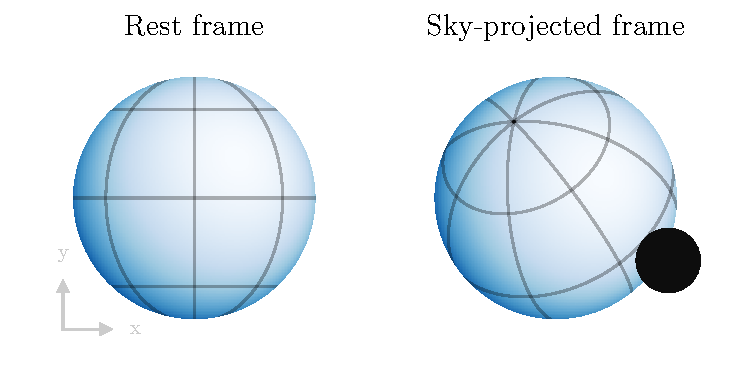
\includegraphics[width=0.6\textwidth]{../workflows/geometry/figures/rotation_basis.pdf}
        \caption{Rotation of a primary body's surface to place it in the sky-projected frame of the observer. \codelink{workflows/geometry/scripts/rotations.ipynb}}
        \label{fig:rotation_basis}
    \end{center}
\end{figure}

The rotation of spherical harmonics involves the computation of Wigner-D-matrices, commonly obtained through robust recursion relations in both degree $l$ and order $m$, but leading to costly computations. Hence, knowing how to decompose the full spherical harmonics rotation using pre-computed rotations is essential to achieve optimal performance in this framework. \autoref{fig:rotation_starry} shows the 6 elementary rotations currently used in \textsf{starry}.
\begin{figure}[H]
    \begin{center}
        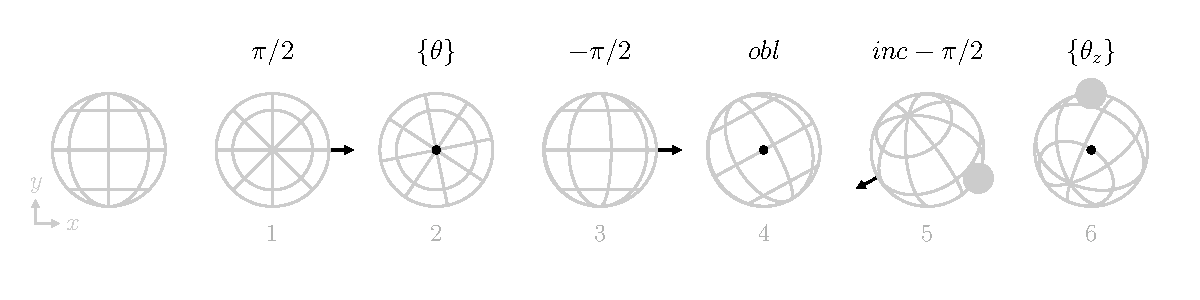
\includegraphics[width=\textwidth]{../workflows/geometry/figures/rotation_starry.pdf}
        \caption{Decomposition of the full rotation of the surface into elementary rotations. Each schematic shows a sphere rotated from a previous orientation around an axis displayed as a black vector and an angle shown on top. \codelink{workflows/geometry/scripts/rotations.ipynb}}
        \label{fig:rotation_starry}
    \end{center}
\end{figure}
In this figure, the first 3 rotations have the effect to rotate the star around its rotation axis, and rotations 3 to 5 place the star on a sky-projected frame. Finally, rotation 6 aligns the spherical harmonics map to the occulting body on the $y$ axis in order to apply Green's theorem in the appropriate basis (Figure 2 from \citealt{starry}).\\\\
The first thing to notice is that rotations 1 to 3 could be simply reduced to a rotation of angle $\theta$ about the y-axis, turning steps 1 to 3 into one. However, rotations around the pole, i.e.\,with a rotation axis along $z$, have simpler expressions that can be implemented separately. In addition, pre-computing these matrices at lower cost is particularly important for steps 2 and 6, involving a potentially large set of angles $\{\theta\}$ and $\{\theta_z\}$, defined over times $\{t\}$, for which to compute the full light curve. This explains the current decomposition of the complete rotation in six separate steps.\\\\
In \textsf{jaxoplanet}, we compute the Wigner-D-matrices by employing the Risbo recursion relations \citep{Risbo1996} implemented in \texttt{JAX} as part of the \texttt{s2fft} Python package \citep{price:s2fft}. In addition, we merge rotations 3, 4 and 5 (see \autoref{fig:rotation_jaxoplanet}) into a single compound rotation of axis
\begin{equation}
    \bvec{v} = \frac{1}{\sqrt{1 - \cos^2{\left(\frac{inc}{2} \right)} \cos^2{\left(\frac{obl}{2}\right)}}} \begin{pmatrix}
        \sin{\left(\frac{inc}{2} \right)} \cos{\left(\frac{obl}{2}\right)}\\
        \sin{\left(\frac{inc}{2} \right)} \sin{\left(\frac{obl}{2}\right)}\\
         - \cos{\left(\frac{inc}{2} \right)} \sin{\left(\frac{obl}{2}\right)}\\
    \end{pmatrix},
\end{equation}
and angle
\begin{equation}
    \label{eq:combined_angle}
    \omega = 2 \cos^{-1}{\left(\cos{\left(\frac{inc}{2} \right)} \cos{\left(\frac{obl}{2}\right)} \right)}.
\end{equation}
This way, the complete rotation reduces to the four separate steps shown in \autoref{fig:rotation_jaxoplanet}.
\begin{figure}[H]
    \begin{center}
        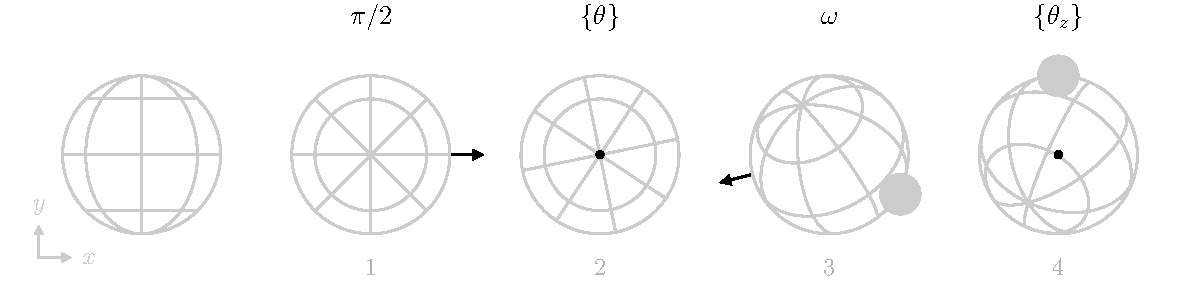
\includegraphics[width=\textwidth]{../workflows/geometry/figures/rotation_jaxoplanet_1.pdf}
        \caption{Consecutive rotations of the spherical harmonics basis in the \textsf{jaxoplanet} implementation. Each schematic shows a sphere rotated from a previous orientation around an axis displayed as a black vector and an angle shown on top. \codelink{workflows/geometry/scripts/rotations.ipynb}}
        \label{fig:rotation_jaxoplanet}
    \end{center}
\end{figure}

\subsection{Computation of the solution vectors}\label{solution_vector}

We described in \autoref{occultation} how the integrated intensity of a spherical body occulted by another can be computed using the solution vector $\bvec{s}^\mathsf{T}$. \cite{pal2012} emphasizes that, knowing $\bvec{G}_n$, each component $s_n$ of the solution vector defined in \autoref{eq:sn_gn} can be decomposed into
\begin{equation}
    s_n = \mathcal{Q}(\bvec{G}_n) - \mathcal{P}(\bvec{G}_n)
\end{equation}
where $\mathcal{Q}(\bvec{G}_n)$ and $\mathcal{P}(\bvec{G}_n)$ are line integrals over the contours of the occulting body and the primary's surface, as shown in \autoref{fig:geometry}.
%
\begin{figure}[H]
    \begin{center}
        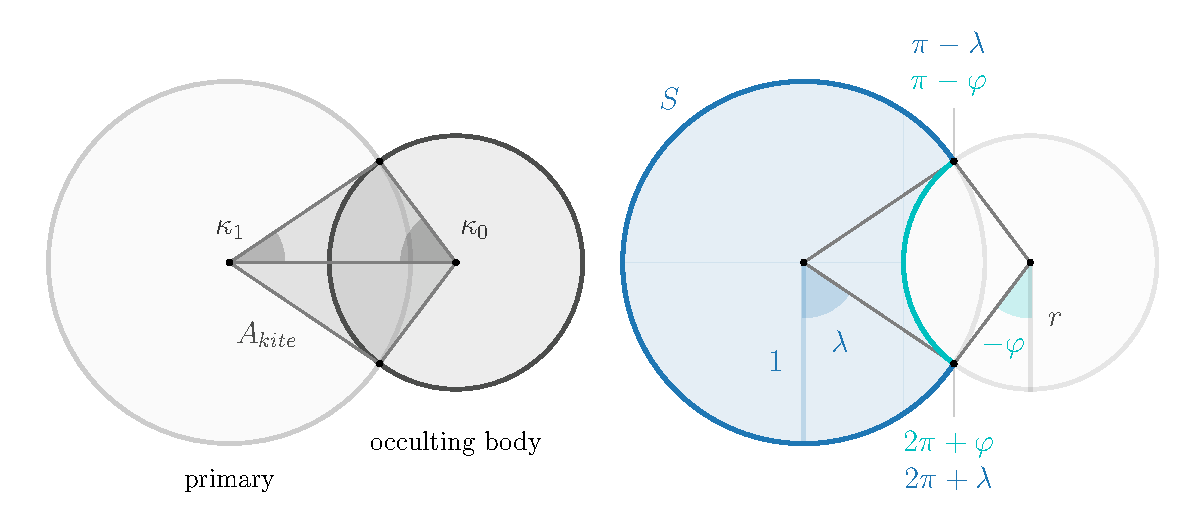
\includegraphics[width=\textwidth]{../workflows/geometry/figures/occultation_geometry.pdf}
        \caption{Geometric configuration and angles definitions for the two-body occultation. On the left figure, the larger light grey disk corresponds to the primary body being occulted by the darker secondary body. On the right figure, the area $S$ over which the intensity is integrated is shown in light blue. By choosing an appropriate transform, the integration over $S$ can be reduced to a line integral over the contour of the occulting body, which can be decomposed into the contour of the occulting body within the area of the primary body (in cyan) and the contour of the primary body everywhere else (in blue). \codelink{workflows/geometry/scripts/occultation_geometry.ipynb}}
        \label{fig:geometry}
    \end{center}
\end{figure}
%
In the general case, the $\mathcal{Q}$ integral (over the blue contour shown in \autoref{fig:geometry}) takes a simple analytical form and can be computed using the recurrence relations from \cite{starry} (Equation D29). The case of a limb-darkened surface is even simpler as $\mathcal{Q}(\bvec{G}_n) = 0$ for all $n > 0$. On the other hand, the $\mathcal{P}$ integral (over the cyan contour shown in \autoref{fig:geometry}) is harder to evaluate and requires the use of recurrence relations and truncated series expansions, with a scheme that depends on the geometric configuration of the system (see \citealt{starry}, Section D.2).\\\\
In order to translate the \textsf{starry}  implementation to \textsf{JAX}, we evaluate the $\mathcal{P}$ integrals numerically using Gauss-Legendre integrations, requiring the evaluation of the integrated functions only over a fixed number of points $q$.\\\\

\subsubsection{Polynomial limb darkening}
For a surface described by a polynomial limb darkening law of order $n$, the $\mathcal{P}$ integral is given in \cite{Agol2020} by
\begingroup\makeatletter\def\f@size{9}\check@mathfonts
$$
    \mbox{\normalsize$\mathcal{P}(\bvec{G}_n)$} =
    \begin{dcases}
        %
        \pi - \kappa_1 - r^2\kappa_0 + \textit{A}_{kite} & \qquad n = 0
        \\[1em]
        \text{see below} & \qquad n = 1
        \\[1em]
        2s_0 + 4\pi\eta - 2\pi & \qquad n = 2
        \\[1em]
        2r(4br)^{\frac{n}{2}}
        \int\displaylimits_{-\kappa_0/2}^{\kappa_0/2}
        (k^2 - \sin^2{\varphi '})^{\frac{n}{2}}
        (r - b + 2b\sin^2\varphi ') \, \text{d}\varphi ' & \qquad \mathrm{n\ge3},
    \end{dcases}
$$
\endgroup
where $\kappa_0$, $\kappa_1$ and $A_{kite}$ are the angles and area shown in \autoref{fig:geometry} and computed following \cite{Agol2020} (Equations 31 and 32). For $n=2$, $\eta$ is defined in \cite{Agol2020} (Equation 53) and depends on the elliptic parameter
%
\begin{equation}
    k = \frac{1-r^2 - b^2 + 2br}{4br},
\end{equation}\\
%
also used in the case $n=3$. For $n=1$, we use Equation 31, 32 and 34 from \cite{starry} to write
%
\begin{equation}
    \mathcal{P}(\bvec{G}_1) = \int\displaylimits_{-\kappa_0/2}^{\kappa_0/2}
        r(r-b\cos{2\varphi '})\;\frac{1-z^3}{3(1-z^2)}\text{d}\varphi ' \quad \text{and} \quad \mathcal{Q}(\bvec{G}_1) = \frac{2}{3}(\pi-\kappa_1),
\end{equation}\\
%
where $1 - z^2 = b + r - 2\cos{\varphi '}$ \footnote{note that $\varphi '$ is different from the angle $\varphi$ shown in \autoref{fig:geometry} and was introduced through the change of variable $\varphi ' = \frac{1}{2}(\varphi -\frac{3\pi}{2})$.}.
\subsubsection{Non-uniform surface}
In the general case, for a star with a non-radially symmetric surface intensity, $n$ denotes the index of the spherical harmonics component such that
\begin{equation}
    n = l^2 + l + m,
\end{equation}
where $l$ is the degree of the spherical harmonic and $m$ its order. For each component, the expression of $\mathcal{P}(\bvec{G}_n)$ depends on $\mu$ and $\nu$ defined as
\begin{equation}
    \begin{aligned}
    \mu &\equiv l - m,\\
    \nu &\equiv l + m.
    \end{aligned}
\end{equation}

The $\mathcal{P}$ integral is then given by Equation D32 from \cite{starry} as
%
\begingroup\makeatletter\def\f@size{9}\check@mathfonts
$$
    \mbox{\normalsize$\mathcal{P}(\bvec{G}_n)$} =
    \begin{dcases}
        %
        2(2r)^{l+2}\int\displaylimits_{-\kappa/2}^{\kappa/2}
            (s_{\varphi '}^2 -s_{\varphi '}^4)^{\frac{\mu+4}{4}}
            (\delta + s_{\varphi '}^2)^{\frac{\nu}{2}}
            \, \text{d}\varphi '
            %
            & \qquad \frac{\mu}{2} \, \mathrm{even}
        \\[1em]
        %
        \mathcal{F}\int\displaylimits_{-\kappa/2}^{\kappa/2}
            (s_{\varphi '}^2-s_{\varphi '}^4)^{\tfrac{l-2}{2}}
            (k^2- s_{\varphi '}^2)^{\frac{3}{2}}
            (1-2s_{\varphi '}^2)
            \, \text{d}\varphi '
            %
            & \qquad \mu = 1, \,
                     l \, \mathrm{even}
        \\[1em]
        %
        \mathcal{F}\int\displaylimits_{-\kappa/2}^{\kappa/2}
            (s_{\varphi '}^2-s_{\varphi '}^4)^{\tfrac{l-3}{2}}
            (\delta + s_{\varphi '}^2)
            (k^2- s_{\varphi '}^2)^{\frac{3}{2}}
            (1-2 s_{\varphi '}^2)
            \, \text{d}\varphi '
            %
            & \qquad \mu = 1, \, l \ne 1, \,
                     l \, \mathrm{odd}
        \\[1em]
        %
        2\mathcal{F}\int\displaylimits_{-\kappa/2}^{\kappa/2}
            (s_{\varphi '}^2-s_{\varphi '}^4)^{\frac{\mu-1}{4}}
            (\delta + s_{\varphi '}^2)^{\frac{\nu-1}{2}}
            (k^2 - s_{\varphi '}^2)^{\frac{3}{2}}
            \, \text{d}\varphi '
            & \qquad \frac{\mu-1}{2} \, \mathrm{even}, \, l \ne 1
        \\[1em]
        %
        \int\displaylimits_{-\kappa/2}^{\kappa/2}
        r(r-b\cos{2\varphi '})\;\frac{1-z^3}{3(1-z^2)}\text{d}\varphi ' & \qquad \mu=1, \, l=1
        \\[1em]
        %
        0 & \qquad \mathrm{otherwise},
    \end{dcases}
$$
\endgroup
%
where $s_{\varphi '} = \sin{\varphi '}$, $\kappa = \varphi + \frac{\pi}{2}$ (see \citealt[Equation D31]{starry}) and $\delta$ is defined for numerical stability as
\begin{equation}
    \delta=\frac{b-r}{2r}.
\end{equation}
Note how, unlike in the \textsf{starry} implementation, the term $\mu=1$, $l=1$ is derived exactly like in the polynomial limb darkening case, instead of analytically which would require the evaluation of elliptic integrals (see \citealt{starry}, Section D.2.3).\\\\
Because of its numerical integration, the precision of the $\mathcal{P}$ integral is limited and depends on the order $q$ of the Gauss-Legendre quadrature, which corresponds to the number of point for which the integrand is evaluated. To minimize this number, we note that all integrands are symmetrical functions, except for $\mu=1$ and $l=1$. Hence, all integrals can be computed over the interval $\left[0, \frac{\kappa}{2}\right]$, instead of $\left[-\frac{\kappa}{2}, \frac{\kappa}{2}\right]$, and multiplied by 2. We also note that all terms for which $\frac{\mu}{2}$ is even reach machine precision for an integration order as low as $q=20$, that we hold fix. With these optimizations, we benchmark the precision and speed of our final implementation for the solution vector in \autoref{performance}.

\subsection{Kepler's equation solver}
\todo{}
\subsection{Light curve functions and transformations}
\todo{}

\section{Performance}\label{performance}
Although occultation light curves have analytical expressions, their practical implementation relies on numerical approximations chosen to balance precision and computation time. This is the case for the solution vector $\bvec{s}^\mathsf{T}$, computed using numerical series expansions in \textsf{starry} (\citealt[section D.2.3]{starry}) and numerical integration in \textsf{jaxoplanet} (see \autoref{solution_vector}). Other expressions, such as the Wigner-D matrices used in the rotation of the spherical harmonics basis, are computed using reccurence relations prone to the accumulation of numerical errors and instability.\\\\
In this section, we evaluate the accuracy and speed of the \textsf{jaxoplanet} implementation and compare it with the C++ implementation of \textsf{starry}.

\subsection{Precision}\label{precision}
We evaluate the precision of the \textsf{starry} and \textsf{jaxoplanet} terms against quantities computed at arbitrary precision, using a ground truth version of the code implemented with the \texttt{mpmath} Python library\footnote{\href{https://mpmath.org/}{https://mpmath.org/}}. The precision of the overall flux $f$ can only be understood by considering the precision of the terms involved in \autoref{eq:starry}: the solution vector $\bvec{s}^\mathsf{T}$ ($\bvec{r}^\mathsf{T}$ if no occultation), the change of basis matrices $\bvec{A_1}$ and $\bvec{A_2}$, and the Wigner-D rotation matrix $\bvec{R}$. Although we show in \autoref{fig:precision_SAR} that the precision of the \textsf{starry} and \textsf{jaxoplanet} implentations slightly differ for many of these terms, we focus this section on the solution vector $\bvec{s}^\mathsf{T}$ and the overall flux $f$.\\\\
Assuming that we perform the numerical integration described in \autoref{solution_vector} at a relatively high order $q=500$, \autoref{fig:precision_s} shows that our reimplentation of \textsf{starry} reaches relative errors lower than 1 part per billion for $\bvec{s}^\mathsf{T}$ and the overall flux $f$, for almost all degrees up to $l_{max}=20$ and considering both a small ($r=0.01$) and a large ($r=100$) occultor transiting the star accross numerically-sensitive values of impact parameters $b$. For reference, \autoref{fig:precision_s_starry} shows comparable errors on the same quantities computed with the C++ implentation of \textsf{starry}. 
\begin{figure}[H]
    \begin{center}
        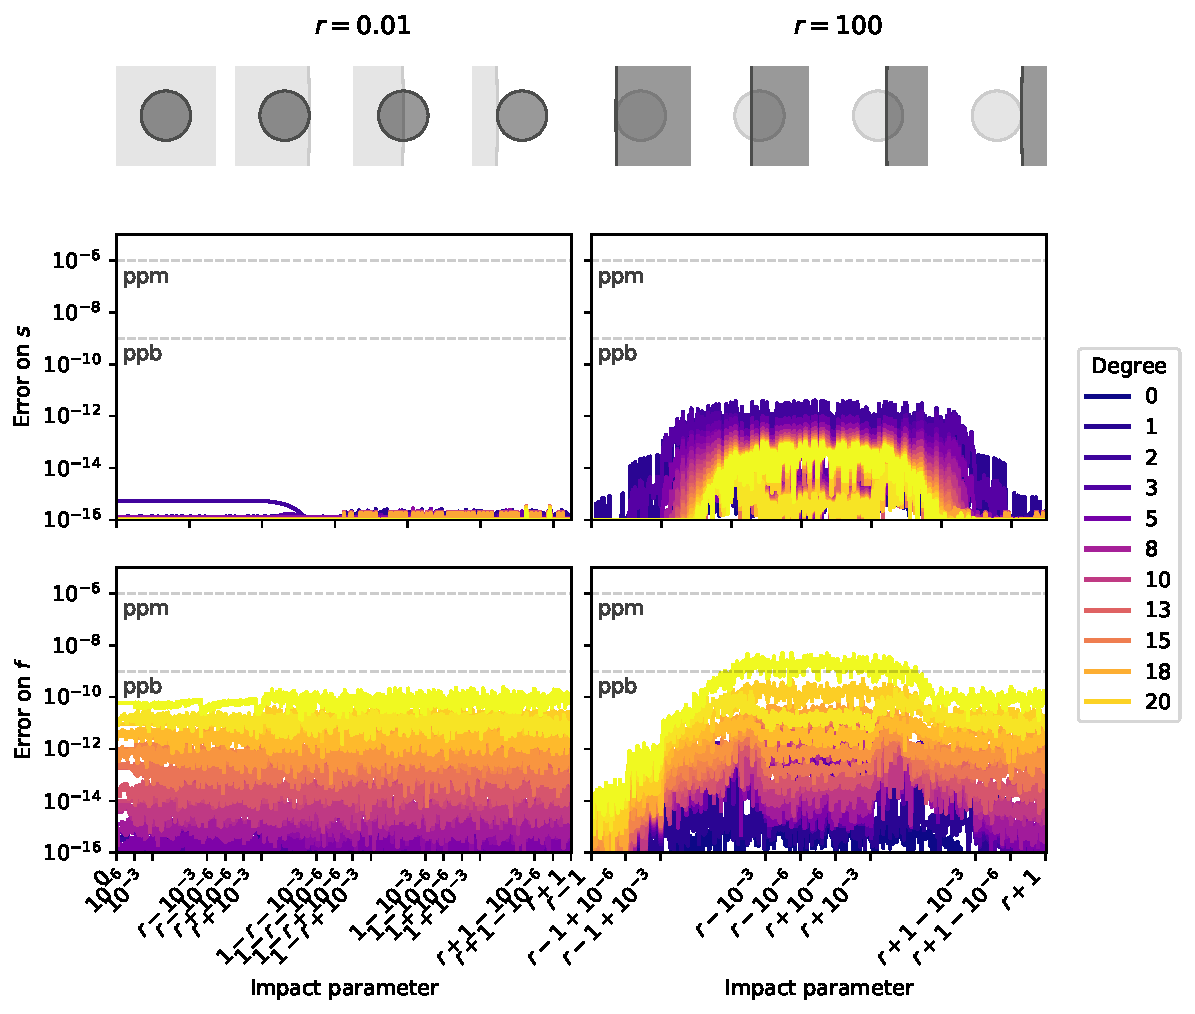
\includegraphics[width=\textwidth]{../workflows/precision/figures/error_jax.pdf}
        \caption{Error of the solution vector $\bvec{s}^\mathsf{T}$ and the overall flux $f$ for all terms of the spherical harmonics basis up to degree $l_{max}=20$. Errors are computed against arbitrary-precision computations of the solution vector and the flux for a small ($r=0.01$) and a large ($r=100$) occultor transiting the star accross numerically-sensitive values of impact parameters $b$. For each basis component $i$, all coefficients are set to zero except $y_i=1$ and errors are scaled to the highest values of $\bvec{s}$ (respectively $f$) over $b$. Then, the plotted errors for each degree $l$ are the maximum of the scaled errors over all $m\in [-l, l]$ components over $b$. The disks at the top of the figure show the transit configurations of the occultor (light dark) and the primary surface (light gray) for different values of $b$. \codelink{workflows/precision/scripts/plot_error}}
        \label{fig:precision_s}
    \end{center}
\end{figure}
In addition, \autoref{fig:precision_degree} shows the evolution of the error on $f$ for increasing degrees of the spherical harmonics for \textsf{starry} and \textsf{jaxoplanet}.
\begin{figure}[H]
    \begin{center}
        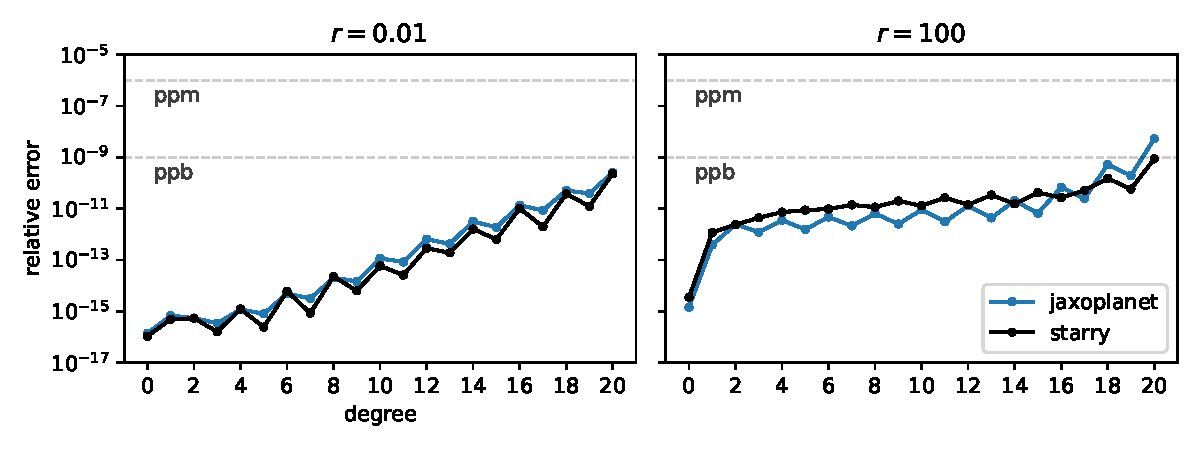
\includegraphics[width=\textwidth]{../workflows/precision/figures/error_degree.pdf}
        \caption{Maximum errors in the overall flux $f$ for all degrees of the spherical harmonics components. Errors shown in this figure correspond to the maximum values of the scaled errors shown in \autoref{fig:precision_s} over the range of values $b$, but computed with $q=250$. \codelink{workflows/precision/scripts/plot_error_vs_degree}}
        \label{fig:precision_degree}
    \end{center}
\end{figure}
In \autoref{fig:precision_limbdark}, we compare the precision of our limb darkened light curve model with \textsf{exoplanet} Python package (which uses the same formalism as \cite{Agol2020} but limited to linear and quadratic limb darkening).from shows the relative error in the flux of a limb-darkened star occulted by an opaque body for increasing orders of a polynomial limb darkening law. In this figure, we also report the error of the flux computed using the \textsf{exoplanet} Python package (which uses the same formalism as \cite{Agol2020} but limited to linear and quadratic limb darkening).
\begin{figure}[H]
    \begin{center}
        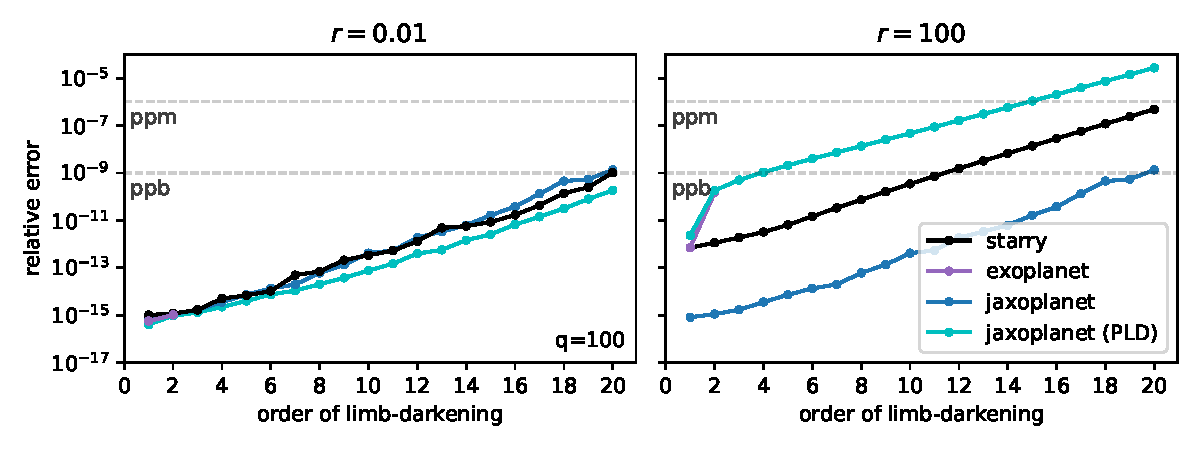
\includegraphics[width=\textwidth]{../workflows/precision/figures/limbdark_error.PDF}
        \caption{Maximum errors in the overall flux $f$ of a star occulted by an opaque body for increasing orders of its polynomial limb darkening law. Errors shown in this figure correspond to the maximum values of the scaled errors shown in \autoref{fig:precision_s} over the range of values $b$, but computed with $q=100$. For each order $n$ all limb darkening coefficients are set to zero except the $n$-th coefficient $u_n=1$. \codelink{workflows/precision/scripts/plot_error_limbdark}}
        \label{fig:precision_limbdark}
    \end{center}
\end{figure}
A set of unitary polynomial limb darkening coefficients of order 20 leads to spherical harmonics coefficients as large as $10^6$. This explains the larger errors observed in \autoref{fig:precision_limbdark} (error versus limb darkening order) compared to the ones shown in \autoref{fig:precision_degree} (error versus degree of the spherical harmonics). We note that the errors scale with the values of $\bvec{u}$.\\\\
With these results, we validate the precision of \textsf{jaxoplanet} and show it is on per with the legacy C++ \textsf{starry} implentation\footnote{version 1.2.0 \citep{starry_120}} described in \cite{starry}.\\\\
As described in \autoref{solution_vector}, we compute occultation light curves using the Gauss Legendre quadrature to approximate the $\mathcal{P}$ integral involved in the expression of the solution vector $\bvec{s}^\mathsf{T}$. Hence, the precision of the computed flux $f$ depends on the order of the Legendre polynomial which defines the number of points used to approximate $\mathcal{P}$. For this reason, users must carefully set the order parameter $q$ to reach the precision required for their application, as shown in \autoref{fig:relative_error_1}.\\\\
\begin{figure}[H]
    \begin{center}
        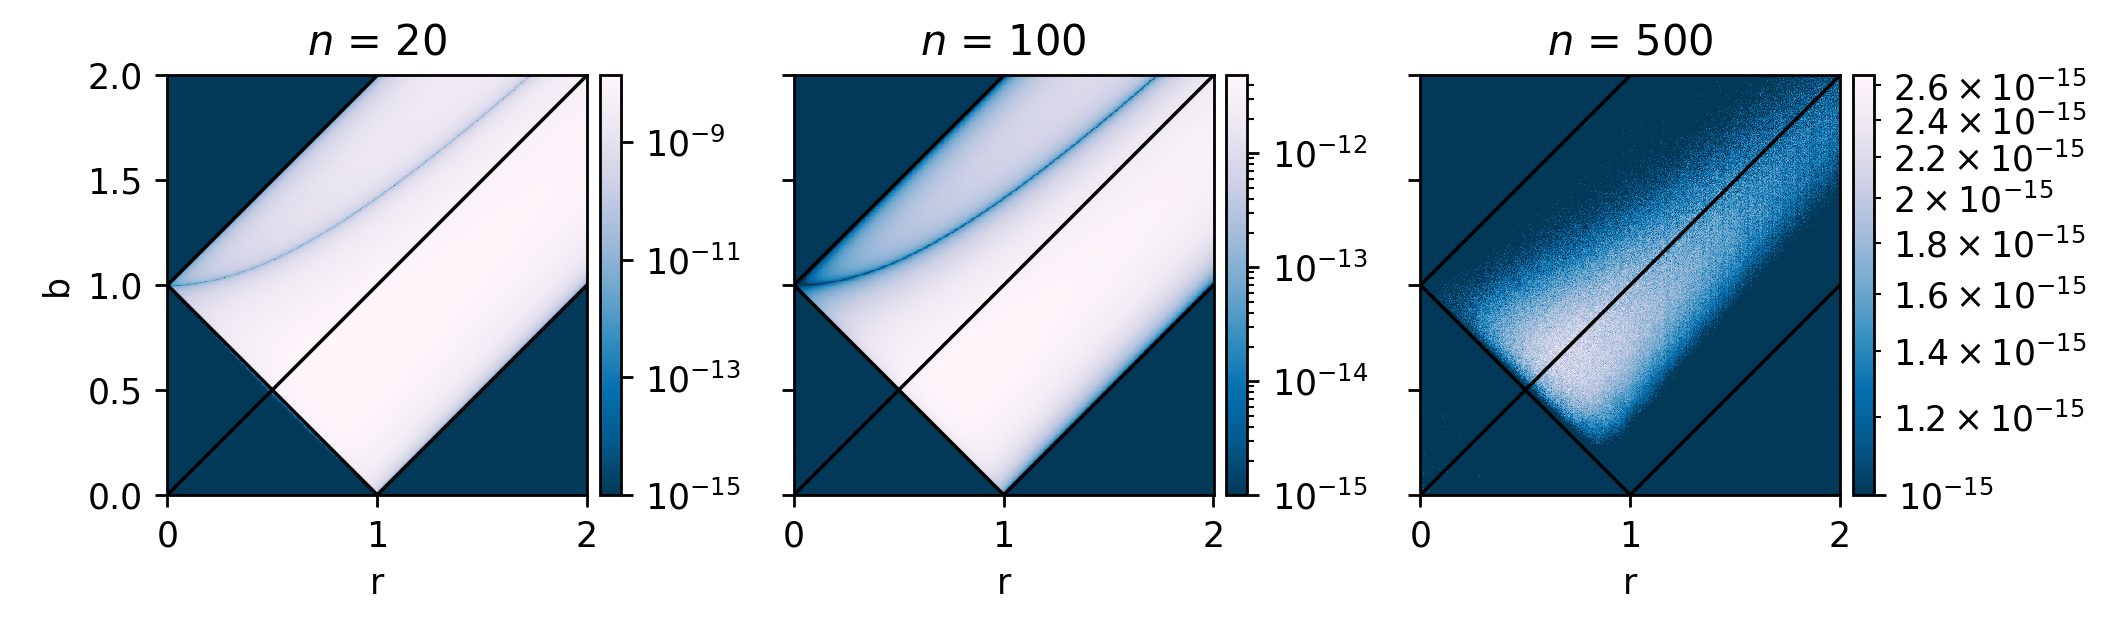
\includegraphics[width=\textwidth]{../workflows/precision/figures/br_error.png}
        \caption{relative numerical error in the flux $f$ of a linearly limb-darkened star (degree $l$=1) transited by an opaque companion over the $(r, b)$ parameter space. The error is evaluated for different orders $q$ of the Gauss-Legendre quadrature and computed against values of $f$ obtained with $q=800$. Note that \autoref{fig:precision_s} was produced using $q=500$ (right plot) for which $\bvec{s}$ reaches machine precision. \codelink{workflows/precision/scripts/plot_br_error}}
        \label{fig:relative_error_1}
    \end{center}
\end{figure}
% In \autoref{fig:precision_order_gausslegendre}, we show how the error in the solution vector evolves with the order $n$ of the Gauss-Legendre quadrature, and its impact on the error in the overall flux.
% \begin{figure}[H]
%     \begin{center}
%         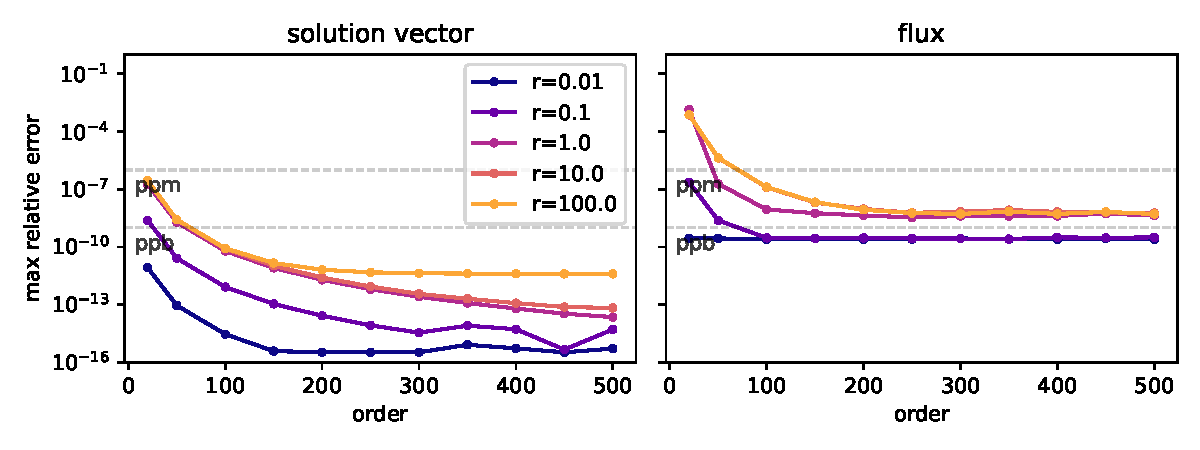
\includegraphics[width=\textwidth]{../workflows/precision/figures/error_order.pdf}
%         \caption{Maximum errors in the solution vector and overall flux $f$ for different occultor radii and orders $n$ of the Gauss-Legendre quadrature used to compute the P integral (see \autoref{solution_vector}). Errors shown in this figure correspond to the maximum values of the scaled errors shown in \autoref{fig:precision_s}, maxima taken over the range of values $b$. As in \autoref{fig:precision_s} the maximum degree of the spherical harmonics basis is set to $l=20$.}
%         \label{fig:precision_order_gausslegendre}
%     \end{center}
% \end{figure}
The minimum error is always achieved for higher values of $q$, which comes with increased computation time (see \autoref{speed}). Hence users must carefully set the order parameter to balance precision and computational speed. As the minimum error reached also depends on the degree of the spherical harmonics basis used, \autoref{fig:precision_order_gausslegendre_degree} shows the errors on the flux for each degree of the spherical harmonics basis, for an occultor with relative radii $r=0.01$, $r=1$ and $r=100$.
\begin{figure}[H]
    \begin{center}
        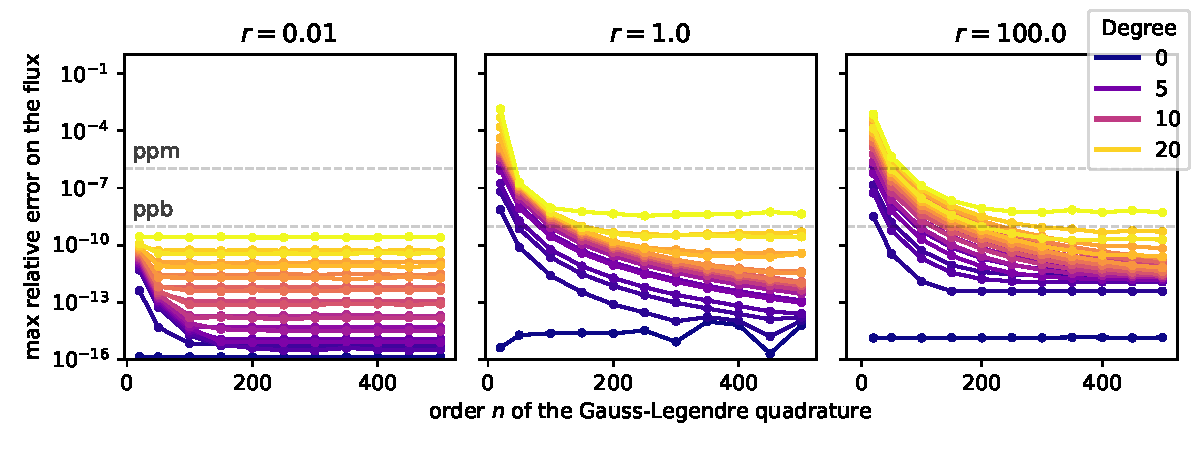
\includegraphics[width=\textwidth]{../workflows/precision/figures/error_order_degree.pdf}
        \caption{Maximum errors in the overall flux $f$ for all degrees of the spherical harmonics components for different occultor radii and orders $q$ of the Gauss-Legendre quadrature used to compute the P integral (see \autoref{solution_vector}). Errors shown in this figure correspond to the maximum values of the scaled errors shown in \autoref{fig:precision_s}, maxima taken over the range of values $b$.}
        \label{fig:precision_order_gausslegendre_degree}
    \end{center}
\end{figure}
\subsection{Speed}\label{speed}

One of the advantage of the \textsf{JAX} library is its ability to perform hardware-accelerated computations on CPUs and GPUs. In this section, we evaluate the speed of the \textsf{jaxoplanet} implementation and compare it with the C++ implementation of \textsf{starry}. For quadratically limb darkened light curves, we also compare our implementation with the one provided by the \textsf{exoplanet} Python package.\\\\
In \autoref{fig:speed_order_gausslegendre}, we show the evolution of the time required to compute the occultation light curve of a limb darkened star and that of a non-uniform star described by spherical harmonics of degree $l_{max}=20$, depending on the order $q$ of the numerical integration. On CPU, our benchmark is done on the single core of an Apple M2 max chip, while on GPU we use the single core of an NVIDIA Tesla V100 processor.\\\\
\begin{figure}[H]
    \begin{center}
        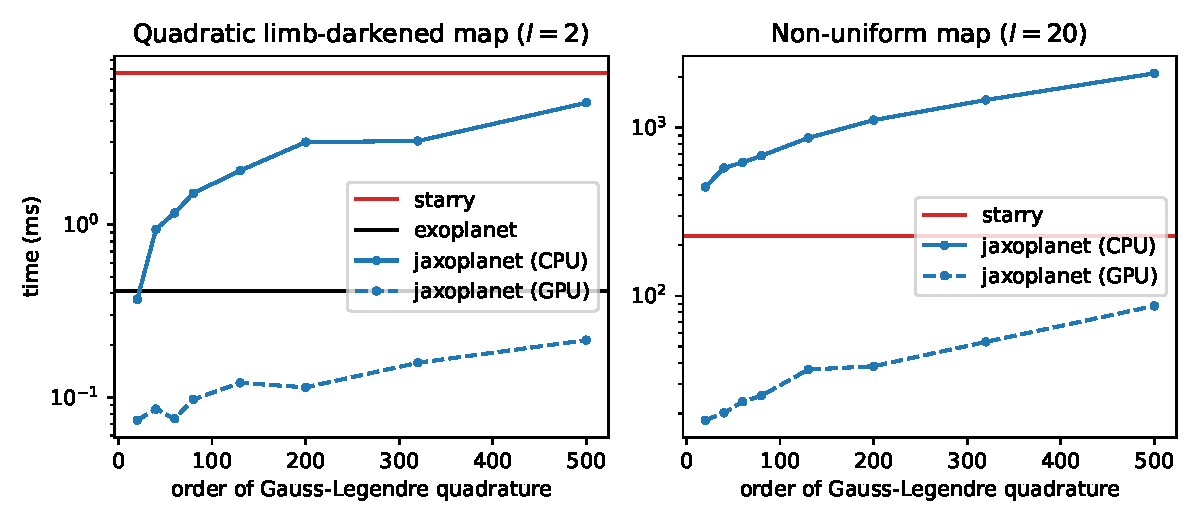
\includegraphics[width=\textwidth]{../workflows/speed/figures/speed_vs_order.pdf}
        \caption{Computation time of the occultation light curve of a limb-darkened star (left) and a non-uniform star described by spherical harmonics up to order $l_{max}=20$ (right) depending on the order $q$ of the Gauss-Legendre quadrature used to compute the $\mathcal{P}$ integral numerically (see \autoref{solution_vector}). The processing time reported for \textsf{exoplanet} and \textsf{starry} is independent of $q$ as these two codes provide closed-form solutions for the integral $\mathcal{P}$. Light curves are computed for $10\,000$ points in transit and an occultor radius $r=0.1$.}
        \label{fig:speed_order_gausslegendre}
    \end{center}
\end{figure}
Finally, \autoref{fig:speed_N} shows the evaluation time of \textsf{jaxoplanet} as a function of the number of points in the light curve compared to \textsf{exoplanet}, for a quadratically limb darkened star, and \textsf{starry}, for a surface map of degree $l_{max} = 20$.
\begin{figure}[H]
    \begin{center}
        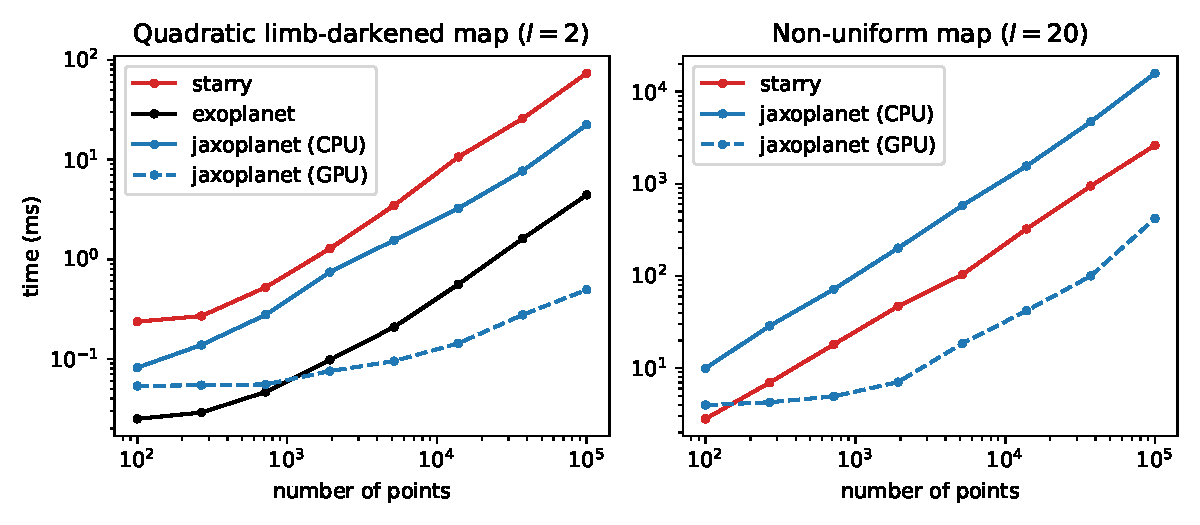
\includegraphics[width=\textwidth]{../workflows/speed/figures/speed_vs_N.pdf}
        \caption{Computation time of the occultation light curve of a limb-darkened star (left) and a non-uniform star described by spherical harmonics up to order $l_{max}=20$ (right) depending on the number of points in the light curve. Light curves are computed at $q=200$ and an occultor radius $r=0.1$.}
        \label{fig:speed_N}
    \end{center}
\end{figure}
These benchmarks are produced for values of $q$ which guarantee that our models reach the same precision as state-of-the-art codes. As discussed in \autoref{discussion}, \textsf{jaxoplanet} can be further optimized by reducing the order $q$ of numerical integration while keeping the precision required for specific applications. In this context, the \textsf{jaxoplanet} Python package provide helper functions to estimate the precision of the light curve model given the relative radius $r$, the spherical harmonics degree $l_{max}$ (if general non-uniform maps are requires), the order of the polynomial limb darkening, and the order $q$ of the numerical integration.\\\\

\section{Discussion}\label{discussion}

In \autoref{precision}, we showed that \textsf{jaxoplanet} is on par with the C++ implementation of \textsf{starry} in terms of precision. As relatively high values of $q$ are required to achieve this performance, results from \autoref{speed} are deceiving and suggest that \textsf{jaxoplanet} is about an order of magnitude slower than \textsf{exoplanet} or \textsf{starry} on CPU, and only advantageous on GPU for very large datasets. Although we expect to further optimize our \textsf{JAX} implementation and bridge this gap in the future, \textsf{jaxoplanet} can currently outperform state-of-the-art codes for most realistic datasets. Indeed, models computed at low values of $q$, which are very fast, match the precision of measurements from modern instruments.\\\\
To demonstrate our point, we first consider the transmission spectroscopy of TRAPPIST-1 b performed with the JWST/NIRISS instrument (GO-2589, \citealt{Lim2023}). These observations reached an estimated precision of 89 ppm for a planet with a relative radius of the order $r\sim0.1$. In this context, numerical integration with an order as low as $q=10$ guarantees that our model reaches a precision of $10^{-16}$, an execution time on par with \textsf{exoplanet} on CPU and up to an order of magnitude faster on GPU for large datasets (see left plot of \autoref{fig:real_benchmark}). The second example we consider is the secondary ecclipse mapping of HD 189733b ($r\sim0.3$) using Spitzer's 8 micron channel \citep{majeau2012} obtained at a precision of about 1 ppt. For a spherical harmonics map of degree $l_{max}=3$ (although $l_{max}=1$ is enough in this case), $q=10$ guarantees a model with a precision of $10^{-10}$, an execution time one order of magnitude faster than \textsf{starry} on CPU and up to two orders of magnitude faster on GPU for large datasets (see right plot of \autoref{fig:real_benchmark}).\\\\
\begin{figure}[H]
    \begin{center}
        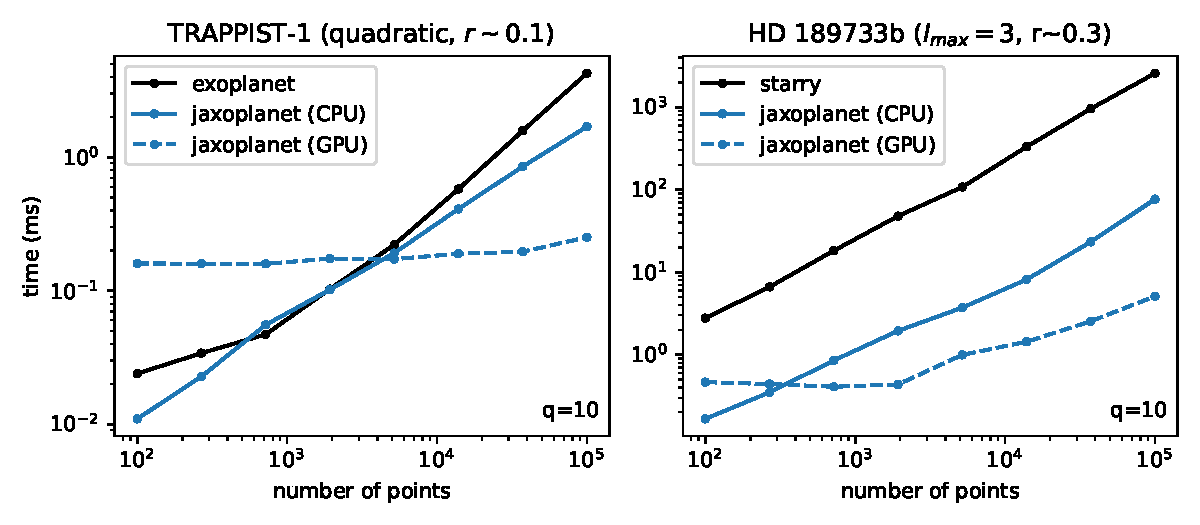
\includegraphics[width=\textwidth]{../workflows/speed/figures/speed_vs_N_realistic.pdf}
        \caption{}
        \label{fig:real_benchmark}
    \end{center}
\end{figure}


\section{Conclusion}
In this paper we presented \textsf{jaxoplanet}, a new implementation of the analytical light curve model \textit{starry} developed using the machine learning library \textsf{JAX}. We showed that our implementation is on par with the legacy C++ \textsf{starry} implementation, and that it offers a significant speed advantage on GPUs for large datasets, enabled by \textsf{JAX}'s just-in-time compilation and hardware acceleration. Our code can be used in association with the large ecosystem of probabilistic and sampling libraries developed in \textsf{JAX}, and will facilitate the development of tools and pipeline for the modeling of TESS and JWST observations, but also future missions such as PLATO \citep{Rauer2014} and ARIEL \citep{Tinetti2018}.\\\\
As the core of our model is developed in Python, we expect \textsf{jaxoplanet} to serve as a basis for the implementation of more complex light curve models, such as light curves of Doppler maps \citep{Luger2021c}, reflected maps \citep{Luger2022}, or non-spherical bodies maps \citep{Dholakia2024}. Eventually, \textsf{jaxoplanet} will take over \textsf{starry} in acting as a foundation to explore and develop analytical methods to numerically reconstruct the surface of exoplanets and stars, deepening our understanding of exoplanetary systems and their worlds.\\\\
The \textsf{jaxoplanet} code is open source under the MIT License and is hosted at \href{https://github.com/exoplanet-dev/jaxoplanet/}{https://github.com/exoplanet-dev/jaxoplanet}, with documentation and tutorials hosted at \href{https://jax.exoplanet.codes}{https://jax.exoplanet.codes}. A permanent version of the code used to generate the figures and results in this paper is archived at https://doi.org/10.5281/zenodo.1312286.


\bibliography{ref}

\appendix

\section{Error budget}
\begin{figure}[H]
    \begin{center}
        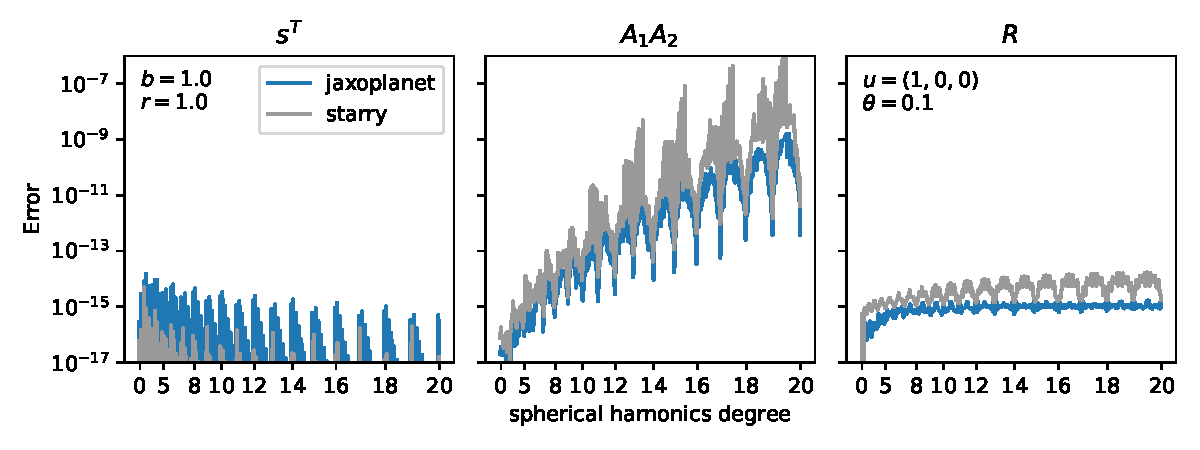
\includegraphics[width=\textwidth]{../workflows/precision/figures/error_SAR.pdf}
        \caption{\codelink{workflows/precision/scripts/plot_error_SAR}}
        \label{fig:precision_SAR}
    \end{center}
\end{figure}

\begin{figure}[H]
    \begin{center}
        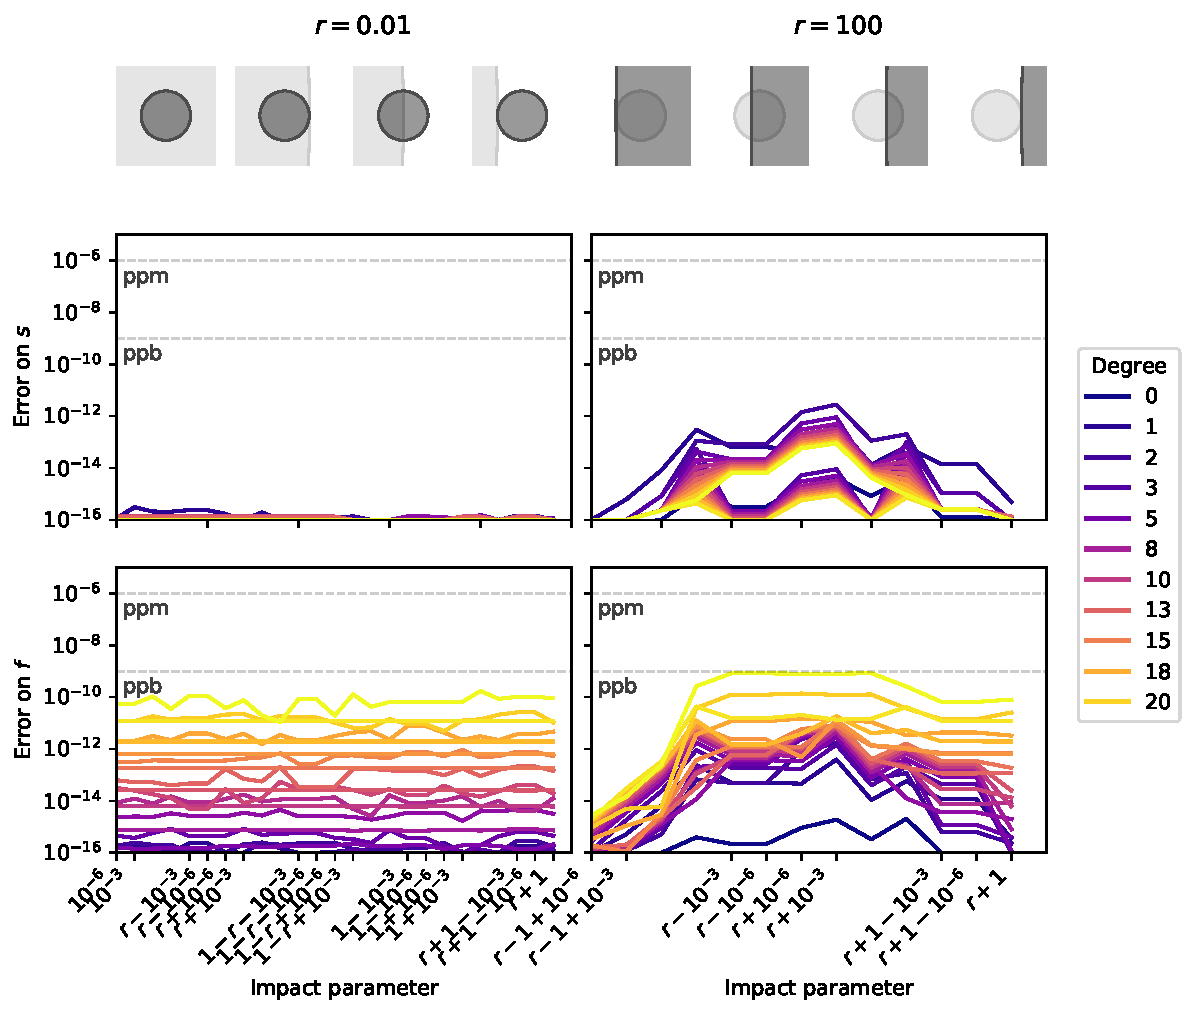
\includegraphics[width=\textwidth]{../workflows/precision/figures/error_starry.pdf}
        \caption{Same as \autoref{fig:precision_s} but with $\bvec{s}^\mathsf{T}$ and $f$ computed with the C++ implementation of \textsf{starry}. \codelink{workflows/precision/scripts/plot_error}}
        \label{fig:precision_s_starry}
    \end{center}
\end{figure}

% Table of symbols

\clearpage
\begin{center}
\renewcommand*{\arraystretch}{1.08}
\begin{longtable}{cll}
\caption{Symbols used in this paper} \label{tab:symbols} \\
%
\toprule
\multicolumn{1}{c}{\textbf{Symbol}} &
\multicolumn{1}{c}{\textbf{Definition}} &
\multicolumn{1}{c}{\textbf{Reference}} \\
\midrule
\endfirsthead
%
\multicolumn{3}{c}%
{{\bfseries \tablename\ \thetable{} --} continued from previous page} \\
\toprule
\multicolumn{1}{c}{\textbf{Symbol}} &
\multicolumn{1}{c}{\textbf{Definition}} &
\multicolumn{1}{c}{\textbf{Reference}} \\
\midrule
\endhead
\bottomrule
%
\endfoot
%
\bottomrule
\endlastfoot
%
$\omega$        & Rotation angle of the combined rotation       & \autoref{eq:combined_angle} \\
$n$ & order of the Gauss-Legendre approximation & \\
$r$ & occultor radius in units of occulted body's radius & \\
%
\end{longtable}
\end{center}

\end{document}